\documentclass{beamer}

\usepackage[utf8x]{inputenc}
\usepackage{fancyvrb}
\usepackage{color}
\usepackage{graphicx}
% \usepackage{wrapfig}
\usepackage{verbatim}

\usetheme{Darmstadt}

\title {Code Coverage and the Definition of Done}
\author{Dénes Mátételki}
\institute{www.emerson.com}
\date{October 2, 2012}

\makeatletter
\def\PY@reset{\let\PY@it=\relax \let\PY@bf=\relax%
    \let\PY@ul=\relax \let\PY@tc=\relax%
    \let\PY@bc=\relax \let\PY@ff=\relax}
\def\PY@tok#1{\csname PY@tok@#1\endcsname}
\def\PY@toks#1+{\ifx\relax#1\empty\else%
    \PY@tok{#1}\expandafter\PY@toks\fi}
\def\PY@do#1{\PY@bc{\PY@tc{\PY@ul{%
    \PY@it{\PY@bf{\PY@ff{#1}}}}}}}
\def\PY#1#2{\PY@reset\PY@toks#1+\relax+\PY@do{#2}}

\expandafter\def\csname PY@tok@gd\endcsname{\def\PY@tc##1{\textcolor[rgb]{0.63,0.00,0.00}{##1}}}
\expandafter\def\csname PY@tok@gu\endcsname{\let\PY@bf=\textbf\def\PY@tc##1{\textcolor[rgb]{0.50,0.00,0.50}{##1}}}
\expandafter\def\csname PY@tok@gt\endcsname{\def\PY@tc##1{\textcolor[rgb]{0.00,0.25,0.82}{##1}}}
\expandafter\def\csname PY@tok@gs\endcsname{\let\PY@bf=\textbf}
\expandafter\def\csname PY@tok@gr\endcsname{\def\PY@tc##1{\textcolor[rgb]{1.00,0.00,0.00}{##1}}}
\expandafter\def\csname PY@tok@cm\endcsname{\let\PY@it=\textit\def\PY@tc##1{\textcolor[rgb]{0.25,0.50,0.50}{##1}}}
\expandafter\def\csname PY@tok@vg\endcsname{\def\PY@tc##1{\textcolor[rgb]{0.10,0.09,0.49}{##1}}}
\expandafter\def\csname PY@tok@m\endcsname{\def\PY@tc##1{\textcolor[rgb]{0.40,0.40,0.40}{##1}}}
\expandafter\def\csname PY@tok@mh\endcsname{\def\PY@tc##1{\textcolor[rgb]{0.40,0.40,0.40}{##1}}}
\expandafter\def\csname PY@tok@go\endcsname{\def\PY@tc##1{\textcolor[rgb]{0.50,0.50,0.50}{##1}}}
\expandafter\def\csname PY@tok@ge\endcsname{\let\PY@it=\textit}
\expandafter\def\csname PY@tok@vc\endcsname{\def\PY@tc##1{\textcolor[rgb]{0.10,0.09,0.49}{##1}}}
\expandafter\def\csname PY@tok@il\endcsname{\def\PY@tc##1{\textcolor[rgb]{0.40,0.40,0.40}{##1}}}
\expandafter\def\csname PY@tok@cs\endcsname{\let\PY@it=\textit\def\PY@tc##1{\textcolor[rgb]{0.25,0.50,0.50}{##1}}}
\expandafter\def\csname PY@tok@cp\endcsname{\def\PY@tc##1{\textcolor[rgb]{0.74,0.48,0.00}{##1}}}
\expandafter\def\csname PY@tok@gi\endcsname{\def\PY@tc##1{\textcolor[rgb]{0.00,0.63,0.00}{##1}}}
\expandafter\def\csname PY@tok@gh\endcsname{\let\PY@bf=\textbf\def\PY@tc##1{\textcolor[rgb]{0.00,0.00,0.50}{##1}}}
\expandafter\def\csname PY@tok@ni\endcsname{\let\PY@bf=\textbf\def\PY@tc##1{\textcolor[rgb]{0.60,0.60,0.60}{##1}}}
\expandafter\def\csname PY@tok@nl\endcsname{\def\PY@tc##1{\textcolor[rgb]{0.63,0.63,0.00}{##1}}}
\expandafter\def\csname PY@tok@nn\endcsname{\let\PY@bf=\textbf\def\PY@tc##1{\textcolor[rgb]{0.00,0.00,1.00}{##1}}}
\expandafter\def\csname PY@tok@no\endcsname{\def\PY@tc##1{\textcolor[rgb]{0.53,0.00,0.00}{##1}}}
\expandafter\def\csname PY@tok@na\endcsname{\def\PY@tc##1{\textcolor[rgb]{0.49,0.56,0.16}{##1}}}
\expandafter\def\csname PY@tok@nb\endcsname{\def\PY@tc##1{\textcolor[rgb]{0.00,0.50,0.00}{##1}}}
\expandafter\def\csname PY@tok@nc\endcsname{\let\PY@bf=\textbf\def\PY@tc##1{\textcolor[rgb]{0.00,0.00,1.00}{##1}}}
\expandafter\def\csname PY@tok@nd\endcsname{\def\PY@tc##1{\textcolor[rgb]{0.67,0.13,1.00}{##1}}}
\expandafter\def\csname PY@tok@ne\endcsname{\let\PY@bf=\textbf\def\PY@tc##1{\textcolor[rgb]{0.82,0.25,0.23}{##1}}}
\expandafter\def\csname PY@tok@nf\endcsname{\def\PY@tc##1{\textcolor[rgb]{0.00,0.00,1.00}{##1}}}
\expandafter\def\csname PY@tok@si\endcsname{\let\PY@bf=\textbf\def\PY@tc##1{\textcolor[rgb]{0.73,0.40,0.53}{##1}}}
\expandafter\def\csname PY@tok@s2\endcsname{\def\PY@tc##1{\textcolor[rgb]{0.73,0.13,0.13}{##1}}}
\expandafter\def\csname PY@tok@vi\endcsname{\def\PY@tc##1{\textcolor[rgb]{0.10,0.09,0.49}{##1}}}
\expandafter\def\csname PY@tok@nt\endcsname{\let\PY@bf=\textbf\def\PY@tc##1{\textcolor[rgb]{0.00,0.50,0.00}{##1}}}
\expandafter\def\csname PY@tok@nv\endcsname{\def\PY@tc##1{\textcolor[rgb]{0.10,0.09,0.49}{##1}}}
\expandafter\def\csname PY@tok@s1\endcsname{\def\PY@tc##1{\textcolor[rgb]{0.73,0.13,0.13}{##1}}}
\expandafter\def\csname PY@tok@sh\endcsname{\def\PY@tc##1{\textcolor[rgb]{0.73,0.13,0.13}{##1}}}
\expandafter\def\csname PY@tok@sc\endcsname{\def\PY@tc##1{\textcolor[rgb]{0.73,0.13,0.13}{##1}}}
\expandafter\def\csname PY@tok@sx\endcsname{\def\PY@tc##1{\textcolor[rgb]{0.00,0.50,0.00}{##1}}}
\expandafter\def\csname PY@tok@bp\endcsname{\def\PY@tc##1{\textcolor[rgb]{0.00,0.50,0.00}{##1}}}
\expandafter\def\csname PY@tok@c1\endcsname{\let\PY@it=\textit\def\PY@tc##1{\textcolor[rgb]{0.25,0.50,0.50}{##1}}}
\expandafter\def\csname PY@tok@kc\endcsname{\let\PY@bf=\textbf\def\PY@tc##1{\textcolor[rgb]{0.00,0.50,0.00}{##1}}}
\expandafter\def\csname PY@tok@c\endcsname{\let\PY@it=\textit\def\PY@tc##1{\textcolor[rgb]{0.25,0.50,0.50}{##1}}}
\expandafter\def\csname PY@tok@mf\endcsname{\def\PY@tc##1{\textcolor[rgb]{0.40,0.40,0.40}{##1}}}
\expandafter\def\csname PY@tok@err\endcsname{\def\PY@bc##1{\setlength{\fboxsep}{0pt}\fcolorbox[rgb]{1.00,0.00,0.00}{1,1,1}{\strut ##1}}}
\expandafter\def\csname PY@tok@kd\endcsname{\let\PY@bf=\textbf\def\PY@tc##1{\textcolor[rgb]{0.00,0.50,0.00}{##1}}}
\expandafter\def\csname PY@tok@ss\endcsname{\def\PY@tc##1{\textcolor[rgb]{0.10,0.09,0.49}{##1}}}
\expandafter\def\csname PY@tok@sr\endcsname{\def\PY@tc##1{\textcolor[rgb]{0.73,0.40,0.53}{##1}}}
\expandafter\def\csname PY@tok@mo\endcsname{\def\PY@tc##1{\textcolor[rgb]{0.40,0.40,0.40}{##1}}}
\expandafter\def\csname PY@tok@kn\endcsname{\let\PY@bf=\textbf\def\PY@tc##1{\textcolor[rgb]{0.00,0.50,0.00}{##1}}}
\expandafter\def\csname PY@tok@mi\endcsname{\def\PY@tc##1{\textcolor[rgb]{0.40,0.40,0.40}{##1}}}
\expandafter\def\csname PY@tok@gp\endcsname{\let\PY@bf=\textbf\def\PY@tc##1{\textcolor[rgb]{0.00,0.00,0.50}{##1}}}
\expandafter\def\csname PY@tok@o\endcsname{\def\PY@tc##1{\textcolor[rgb]{0.40,0.40,0.40}{##1}}}
\expandafter\def\csname PY@tok@kr\endcsname{\let\PY@bf=\textbf\def\PY@tc##1{\textcolor[rgb]{0.00,0.50,0.00}{##1}}}
\expandafter\def\csname PY@tok@s\endcsname{\def\PY@tc##1{\textcolor[rgb]{0.73,0.13,0.13}{##1}}}
\expandafter\def\csname PY@tok@kp\endcsname{\def\PY@tc##1{\textcolor[rgb]{0.00,0.50,0.00}{##1}}}
\expandafter\def\csname PY@tok@w\endcsname{\def\PY@tc##1{\textcolor[rgb]{0.73,0.73,0.73}{##1}}}
\expandafter\def\csname PY@tok@kt\endcsname{\def\PY@tc##1{\textcolor[rgb]{0.69,0.00,0.25}{##1}}}
\expandafter\def\csname PY@tok@ow\endcsname{\let\PY@bf=\textbf\def\PY@tc##1{\textcolor[rgb]{0.67,0.13,1.00}{##1}}}
\expandafter\def\csname PY@tok@sb\endcsname{\def\PY@tc##1{\textcolor[rgb]{0.73,0.13,0.13}{##1}}}
\expandafter\def\csname PY@tok@k\endcsname{\let\PY@bf=\textbf\def\PY@tc##1{\textcolor[rgb]{0.00,0.50,0.00}{##1}}}
\expandafter\def\csname PY@tok@se\endcsname{\let\PY@bf=\textbf\def\PY@tc##1{\textcolor[rgb]{0.73,0.40,0.13}{##1}}}
\expandafter\def\csname PY@tok@sd\endcsname{\let\PY@it=\textit\def\PY@tc##1{\textcolor[rgb]{0.73,0.13,0.13}{##1}}}

\def\PYZbs{\char`\\}
\def\PYZus{\char`\_}
\def\PYZob{\char`\{}
\def\PYZcb{\char`\}}
\def\PYZca{\char`\^}
\def\PYZam{\char`\&}
\def\PYZlt{\char`\<}
\def\PYZgt{\char`\>}
\def\PYZsh{\char`\#}
\def\PYZpc{\char`\%}
\def\PYZdl{\char`\$}
\def\PYZti{\char`\~}
% for compatibility with earlier versions
\def\PYZat{@}
\def\PYZlb{[}
\def\PYZrb{]}


\makeatother



\begin{document}

%----------- slide --------------------------------------------------%

\begin{frame}
% \titlepage
\begin{titlepage}
\begin{center}

\includegraphics[height=3.3cm]{qr_cc_and_dod.png}
\end{center}
\end{titlepage}
% \end{center}

\end{frame}

%----------- slide --------------------------------------------------%

\begin{frame}
\frametitle{Table of contents}
\tableofcontents
\end{frame}

%----------- slide --------------------------------------------------%

\section{Definitions}

% \subsection{Testing}
\subsection{Legacy code}

%----------- slide --------------------------------------------------%

\begin{frame}{Legacy code, unit test, functional test}



\begin{block}{Legacy code}
% \small
"Code without tests is bad code. It doesn't matter how well written it is; it doesn't matter how pretty or object-oriented or well-encapsulated it is. With tests, we can change the behaviour of our code quickly and verifiably. Without them, we really don't know if our code is getting better or worse." \cite{legacy}
\end{block}

\end{frame}

%----------- slide --------------------------------------------------%

\subsection{Tests}

\begin{frame}{Legacy code, unit test, functional test}

% \subsection{Unit test}



\begin{block}{Unit Test (UT) - white box testing}
% \small
"The goal of unit testing is to isolate each part of the program and show that the individual parts are correct. A unit test provides a strict, written \textcolor{red}{contract} \cite{dbc} that the piece of code must satisfy." \cite{ut}
\end{block}

% \subsection{Functional test}

\begin{block}{Functional Test (FT) - black box testing}
% \small
"Bases its test cases on the specifications of the software component under test. Functions are tested by feeding them input and examining the output, and internal program structure is rarely considered." \cite{ft}
\end{block}

\end{frame}

%----------- slide --------------------------------------------------%

\subsection{Definition of Done,  Continuous Integration}

\begin{frame}{Definition of Done, Continuous Integration}

\begin{block}{Definition of Done - DoD}
\small
\begin{itemize}
  \item "A checklist of valuable activities required to produce software." \cite{dod} 
% "Writing code, coding comments, unit testing, integration testing, release notes, design documents, etc"
  \item "Different DoD at various levels: feature, sprint, release."
  \item Each team come up with their own DoD which is reviewed and updated as needed.
%   \item Example: unit tests cover > 90\% lines of the code
\end{itemize}
\end{block}

% \subsection{Continuous Integration}

\begin{block}{Continuous Integration - CI}
\small
"Implements continuous processes of applying quality control - small pieces of effort, applied frequently." \cite{ci}

\begin{itemize}
  \item Automate the build.
  \item Make the build self-testing.
%   \item Everyone can see the results of the latest build.
  \item ...verifies the DoD.
\end{itemize}
\end{block}

\end{frame}


\section{Code coverage}

\subsection{gcov and gprof}


%----------- slide --------------------------------------------------%

\begin{frame}{gcov and gprof}

\begin{block}{gcov}
\small
"gcov is a tool you can use in conjunction with GCC to test code coverage in your programs." \cite{gcov}

\begin{itemize}
  \item How often each line of code executes.
  \item Which lines of code are actually executed.
\end{itemize}
\end{block}

% \subsection{gprof}

\begin{block}{gprof}
\small
The GNU profiler. \cite{gprof}

\begin{itemize}
  \item How much computing time each section of code uses.
  \item Can be used with gcov to locate costy algorithms.
\end{itemize}
\end{block}

\end{frame}


%----------- slide --------------------------------------------------%

\subsection{How gcov works}

\begin{frame}{How gcov works}

\begin{block}{gcno}
\small

"The .gcno notes file is generated when the source file is compiled with the GCC \textcolor{red}{-ftest-coverage} option. It contains information to reconstruct the basic block graphs and assign source line numbers to blocks."

\end{block}

\begin{block}{gcda}
\small

"The .gcda count data file is generated when a program containing object files built with the GCC \textcolor{red}{-fprofile-arcs} option is executed. A separate .gcda file is created for each object file compiled with this option. It contains arc transition counts, value profile counts, and some summary information."

\end{block}

\end{frame}

%----------- slide --------------------------------------------------%

\subsection{Example}

\begin{frame}[fragile]{Example}

\begin{exampleblock}{compile and execute}
\tiny
\begin{Verbatim}[numbers=left,firstnumber=1,stepnumber=1]
gcc -fprofile-arcs -ftest-coverage  tmp.c
./a.out
gcov tmp.c
\end{Verbatim}
\end{exampleblock}

\begin{columns}[t]
 
\column{1.5in}

\begin{exampleblock}{tmp.c}
\tiny
\begin{Verbatim}[commandchars=\\\{\},numbers=left,firstnumber=1,stepnumber=1]
\PY{c+cp}{\PYZsh{}}\PY{c+cp}{include \PYZlt{}stdio.h\PYZgt{}}

\PY{k+kt}{int} \PY{n+nf}{main} \PY{p}{(}\PY{k+kt}{void}\PY{p}{)}
\PY{p}{\PYZob{}}
  \PY{k+kt}{int} \PY{n}{i}\PY{p}{,} \PY{n}{total}\PY{p}{;}
  \PY{n}{total} \PY{o}{=} \PY{l+m+mi}{0}\PY{p}{;}
  \PY{k}{for} \PY{p}{(}\PY{n}{i} \PY{o}{=} \PY{l+m+mi}{0}\PY{p}{;} \PY{n}{i} \PY{o}{\PYZlt{}} \PY{l+m+mi}{10}\PY{p}{;} \PY{n}{i}\PY{o}{+}\PY{o}{+}\PY{p}{)}
    \PY{n}{total} \PY{o}{+}\PY{o}{=} \PY{n}{i}\PY{p}{;}

  \PY{k}{if} \PY{p}{(}\PY{n}{total} \PY{o}{!}\PY{o}{=} \PY{l+m+mi}{45}\PY{p}{)}
    \PY{n}{printf} \PY{p}{(}\PY{l+s}{"}\PY{l+s}{Failure}\PY{l+s+se}{\PYZbs{}n}\PY{l+s}{"}\PY{p}{)}\PY{p}{;}
  \PY{k}{else}
    \PY{n}{printf} \PY{p}{(}\PY{l+s}{"}\PY{l+s}{Success}\PY{l+s+se}{\PYZbs{}n}\PY{l+s}{"}\PY{p}{)}\PY{p}{;}
  \PY{k}{return} \PY{l+m+mi}{0}\PY{p}{;}
\PY{p}{\PYZcb{}}
\end{Verbatim}
\end{exampleblock}

\column{2in}

\begin{exampleblock}{gcov output}
\tiny
\begin{Verbatim}[numbers=left,firstnumber=1,stepnumber=1]
    -:    1:#include <stdio.h>
    -:    2:
    1:    3:int main (void)
    -:    4:{
    -:    5:  int i, total;
    1:    6:  total = 0;
   11:    7:  for (i = 0; i < 10; i++)
   10:    8:    total += i;
    -:    9:
    1:   10:  if (total != 45)
#####:   11:    printf ("Failure\n");
    -:   12:  else
    1:   13:    printf ("Success\n");
    1:   14:  return 0;
    -:   15:}
\end{Verbatim}
\end{exampleblock}

\end{columns}

\end{frame}

%----------- slide --------------------------------------------------%

\begin{frame}{Notes and pitfalls}

\begin{block}{Note}
\small

\begin{itemize}
  \item You can combine the results of many runs into one gcda data.
  \item UTs' and FTs' results can be combined too.
\end{itemize}
\end{block}


\begin{block}{Watch out}
\small

\begin{itemize}
  \item "You should compile your code without optimization."
  \item "It works best with a programming style that uses only one statement per line."
  \item "Inlineable functions can create unexpected line counts."
\end{itemize}
\end{block}

\end{frame}

%----------- slide --------------------------------------------------%

\subsection{lcov}

\begin{frame}[fragile]{lcov}

\begin{block}{lcov}
\small
"LCOV is a graphical front-end for GCC's coverage testing tool gcov. It collects gcov data for multiple source files and creates HTML pages containing the source code annotated with coverage information. It also adds overview pages for easy navigation within the file structure." \cite{lcov}
\end{block}

\begin{exampleblock}{compile and execute}
\tiny
\begin{Verbatim}[numbers=left,firstnumber=1,stepnumber=1]
gcc -fprofile-arcs -ftest-coverage  tmp.c
./a.out
lcov --directory . --capture -o lcov.info
mkdir cov
genhtml lcov.info  --frames -o ./cov 
\end{Verbatim}
\end{exampleblock}

\end{frame}

%----------- slide --------------------------------------------------%

\begin{frame}{lcov picture - overview}

\begin{center}
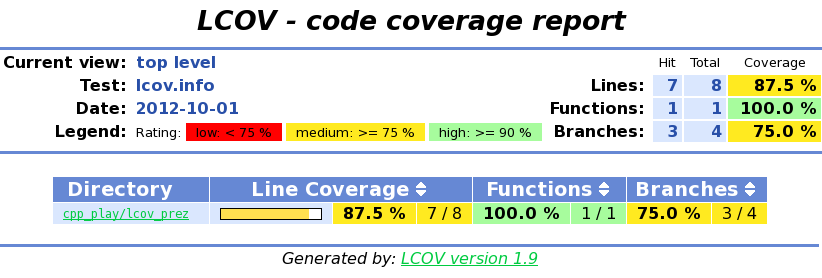
\includegraphics[height=3.6cm]{tmp_c_lcov_overview.png}
\end{center}

\end{frame}

%----------- slide --------------------------------------------------%

\begin{frame}{lcov picture - source browser}

\begin{center}
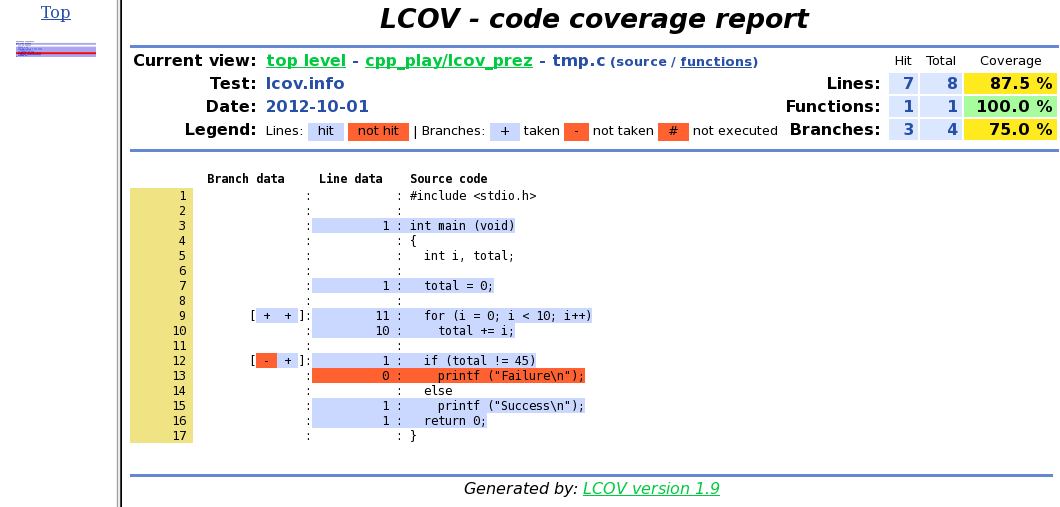
\includegraphics[height=5cm]{tmp_c_lcov_source.png}
\end{center}

\end{frame}

%----------- slide --------------------------------------------------%

\section{Final thoughts}

\subsection{What have we got actually}

\begin{frame}{Final thoughts}

\begin{block}{What have we got actually}
\small
\begin{itemize}
  \item How often each line of code executes.
  \item What are the untested parts.
  \item Dead code detection.
\end{itemize}
\end{block}

\begin{block}{Line testing != funtionality testing}
\small
\begin{itemize}
  \item UTs report code correctness.
  \item CC reports...UT correctness?
\end{itemize}
It's easy to write meaningless UTs to raise CC...it is not enough by itself.
\end{block}

\end{frame}

%----------- slide --------------------------------------------------%

\subsection{CC and Dod}

\begin{frame}{Final thoughs}

\begin{block}{Testing}
\small

\begin{itemize}
%   \item FTs can be written by a "test team" which is sometimes the specification team.
  \item UTs can be written with Test Driven Development - TDD \cite{tdd}
  \item Test and code writer better be a different person otherwise if the code writer misunderstood the requirement, he tests his false model.
  \item Review tests, not just code. Test code quality should meet the same level as code quality.
  \item Test plan and test documentation.
\end{itemize}
\end{block}

\begin{block}{CC as a part of the DoD}
\small

\begin{itemize}
  \item The team agrees on testing principles.
  \item CC should be \textgreater X\%  
  \item This rule can be enforced by CI: build fails if CC \textless X\%.
\end{itemize}
\end{block}

\end{frame}

%----------- slide --------------------------------------------------%

\begin{frame}{Links}

% \begin{wrapfigure}{r}{2cm}



\tiny
\begin{thebibliography}{100}

\bibitem{legacy}
Michael C. Feathers, \emph{Working Effectively with Legacy Code} Prentice Hall, 2004 ISBN 0-13-117705-2

\bibitem{dbc}
\url{http://en.wikipedia.org/wiki/Design_by_contract}

\bibitem{ut}
Kolawa, Adam; Huizinga, Dorota (2007). \emph{Automated Defect Prevention: Best Practices in Software Management} Wiley-IEEE Computer Society Press. p. 426. ISBN 0-470-04212-5.

\bibitem{ft}
Kaner, Falk, Nguyen. \emph{Testing Computer Software} Wiley Computer Publishing, 1999, p. 42. ISBN 0-471-35846-0.

\bibitem{dod}
\url{http://www.scrumalliance.org/articles/105-what-is-definition-of-done-dod}

\bibitem{ci}
\url{http://en.wikipedia.org/wiki/Continuous_integration}

\bibitem{gcov}
\url{http://gcc.gnu.org/onlinedocs/gcc/Gcov.html}

\bibitem{gprof}
\url{http://www.cs.utah.edu/dept/old/texinfo/as/gprof_toc.html}

\bibitem{lcov}
\url{http://ltp.sourceforge.net/coverage/lcov.php}

\bibitem{tdd}
\url{http://en.wikipedia.org/wiki/Test-driven_development}

\end{thebibliography}
\end{frame}

%----------- slide --------------------------------------------------%

%----------- slide --------------------------------------------------%

\begin{frame}{Thank you for your attention!}

\begin{center}

This presentation can be found at: 

\small
\url{http://github.com/cs0rbagomba/cc_and_dod/cc_and_dod.pdf}

\smallskip 
or
\smallskip


\includegraphics[height=3.3cm]{qr_cc_and_dod.png}

\smallskip

Any questions?
\end{center}


\end{frame}

%----------- slide --------------------------------------------------%

\end{document}
